\documentclass[a4paper]{article}

% Includes packages relevant to Senior Lab

% character set specifications
\usepackage[english]{babel}
\usepackage[utf8]{inputenc}

% increased vertical spacing for tables
\newcommand\topVspace{\rule{0pt}{2.6ex}}      
\newcommand\bottomVspace{\rule[-1.2ex]{0pt}{0pt}} 

% extra unicode characters
\DeclareUnicodeCharacter{3BC}{\(\mu\)}
\DeclareUnicodeCharacter{3C1}{\(\rho\)}
\DeclareUnicodeCharacter{2080}{\(_0\)}
\DeclareUnicodeCharacter{2081}{\(_1\)}
\DeclareUnicodeCharacter{2082}{\(_2\)}
\DeclareUnicodeCharacter{3B5}{\(\epsilon\)}
\DeclareUnicodeCharacter{3B1}{\(\alpha\)}

% SI Units
\usepackage{siunitx}

% extra SI units
\DeclareSIUnit\gauss{G}

% enable scientific notation
\sisetup{scientific-notation = engineering, exponent-to-prefix}

% draw pretty lines
\usepackage{tikz}
\usetikzlibrary{datavisualization}
\usepackage{circuitikz}

% manual tabbing
\setlength{\parindent}{0pt}
\def\qq{\qquad}

% include graphics
\usepackage{graphicx}

% increased control over figure placement
\usepackage{float}

% box answers
\usepackage{tcolorbox}

% enable multiple section levels
\usepackage{titlesec}

% define `\subsubsubsection` command
\titleclass{\subsubsubsection}{straight}[\subsection]
\newcounter{subsubsubsection}[subsubsection]
\renewcommand\thesubsubsubsection{\thesubsubsection.\arabic{subsubsubsection}}
\titleformat{\subsubsubsection}
        {\normalfont\normalsize\bfseries}{\thesubsubsubsection}{1em}{}
\titlespacing*{\subsubsubsection}
{0pt}{3.25ex plus 1ex minus .2ex}{1.5ex plus .2ex}
\setcounter{secnumdepth}{4}

% get align environment (among other things)
\usepackage{amsmath}

% bold in math mode
\usepackage{bm}

% get \mathbb (among other things)
\usepackage{amssymb}

\usepackage{array}

% plotting
\usepackage{pgfplots}

% enable external references
\usepackage{hyperref}

% include code
\usepackage[cache=false]{minted}
\setminted{linenos, frame=lines, texcomments}

% adjust margins of individual pages (for shoving figures into place)
\usepackage{changepage}

% rotate figures
\usepackage{rotating}


\usepackage{caption}
\renewcommand{\thetable}{\arabic{section}.\arabic{table}}
\newcommand\T{\rule{0pt}{2.6ex}}       % Top strut
\newcommand\B{\rule[-1.2ex]{0pt}{0pt}} % Bottom strut

\title{PHY 4210-01 Senior Lab \\Lab P1: Planck's Constant\\Lab P6: Blackbody Radiation}

\author{Sarah Arends \\
        Jacquelyne Miksanek \\
        Ryan Wojtyla \\ \\
        Instructor: Dr. Marcus Hohlmann}

\date{\today}

\begin{document}
\maketitle

\begin{abstract}
%physics of experiment
%apparatus used
%what was measured
%Results
\qq 
\end{abstract}

\newpage

\tableofcontents

\newpage

P1 Planck's Constant Experiment

\newpage

\section{Objective of the Experiment}
%A brief statement on the main purpose of the experiment
\qq 

\section{Theory of the Experiment}


\section{Equipment Utilized}
%List principal pieces of apparatus used by manufacturer, model and
%serial number. When it may be important, list principal
%specifications of certain pieces of equipment (e.g. the focal length
%of an optical system, etc.)

% Description of set-up in prose
\qq 

% List of specs
\begin{itemize}
\item itemName \\
\item itemName \\
\end{itemize}

%Labeled sketch of the experimental setup
\begin{figure}[H]
\centering
% uncomment the line below to add image
%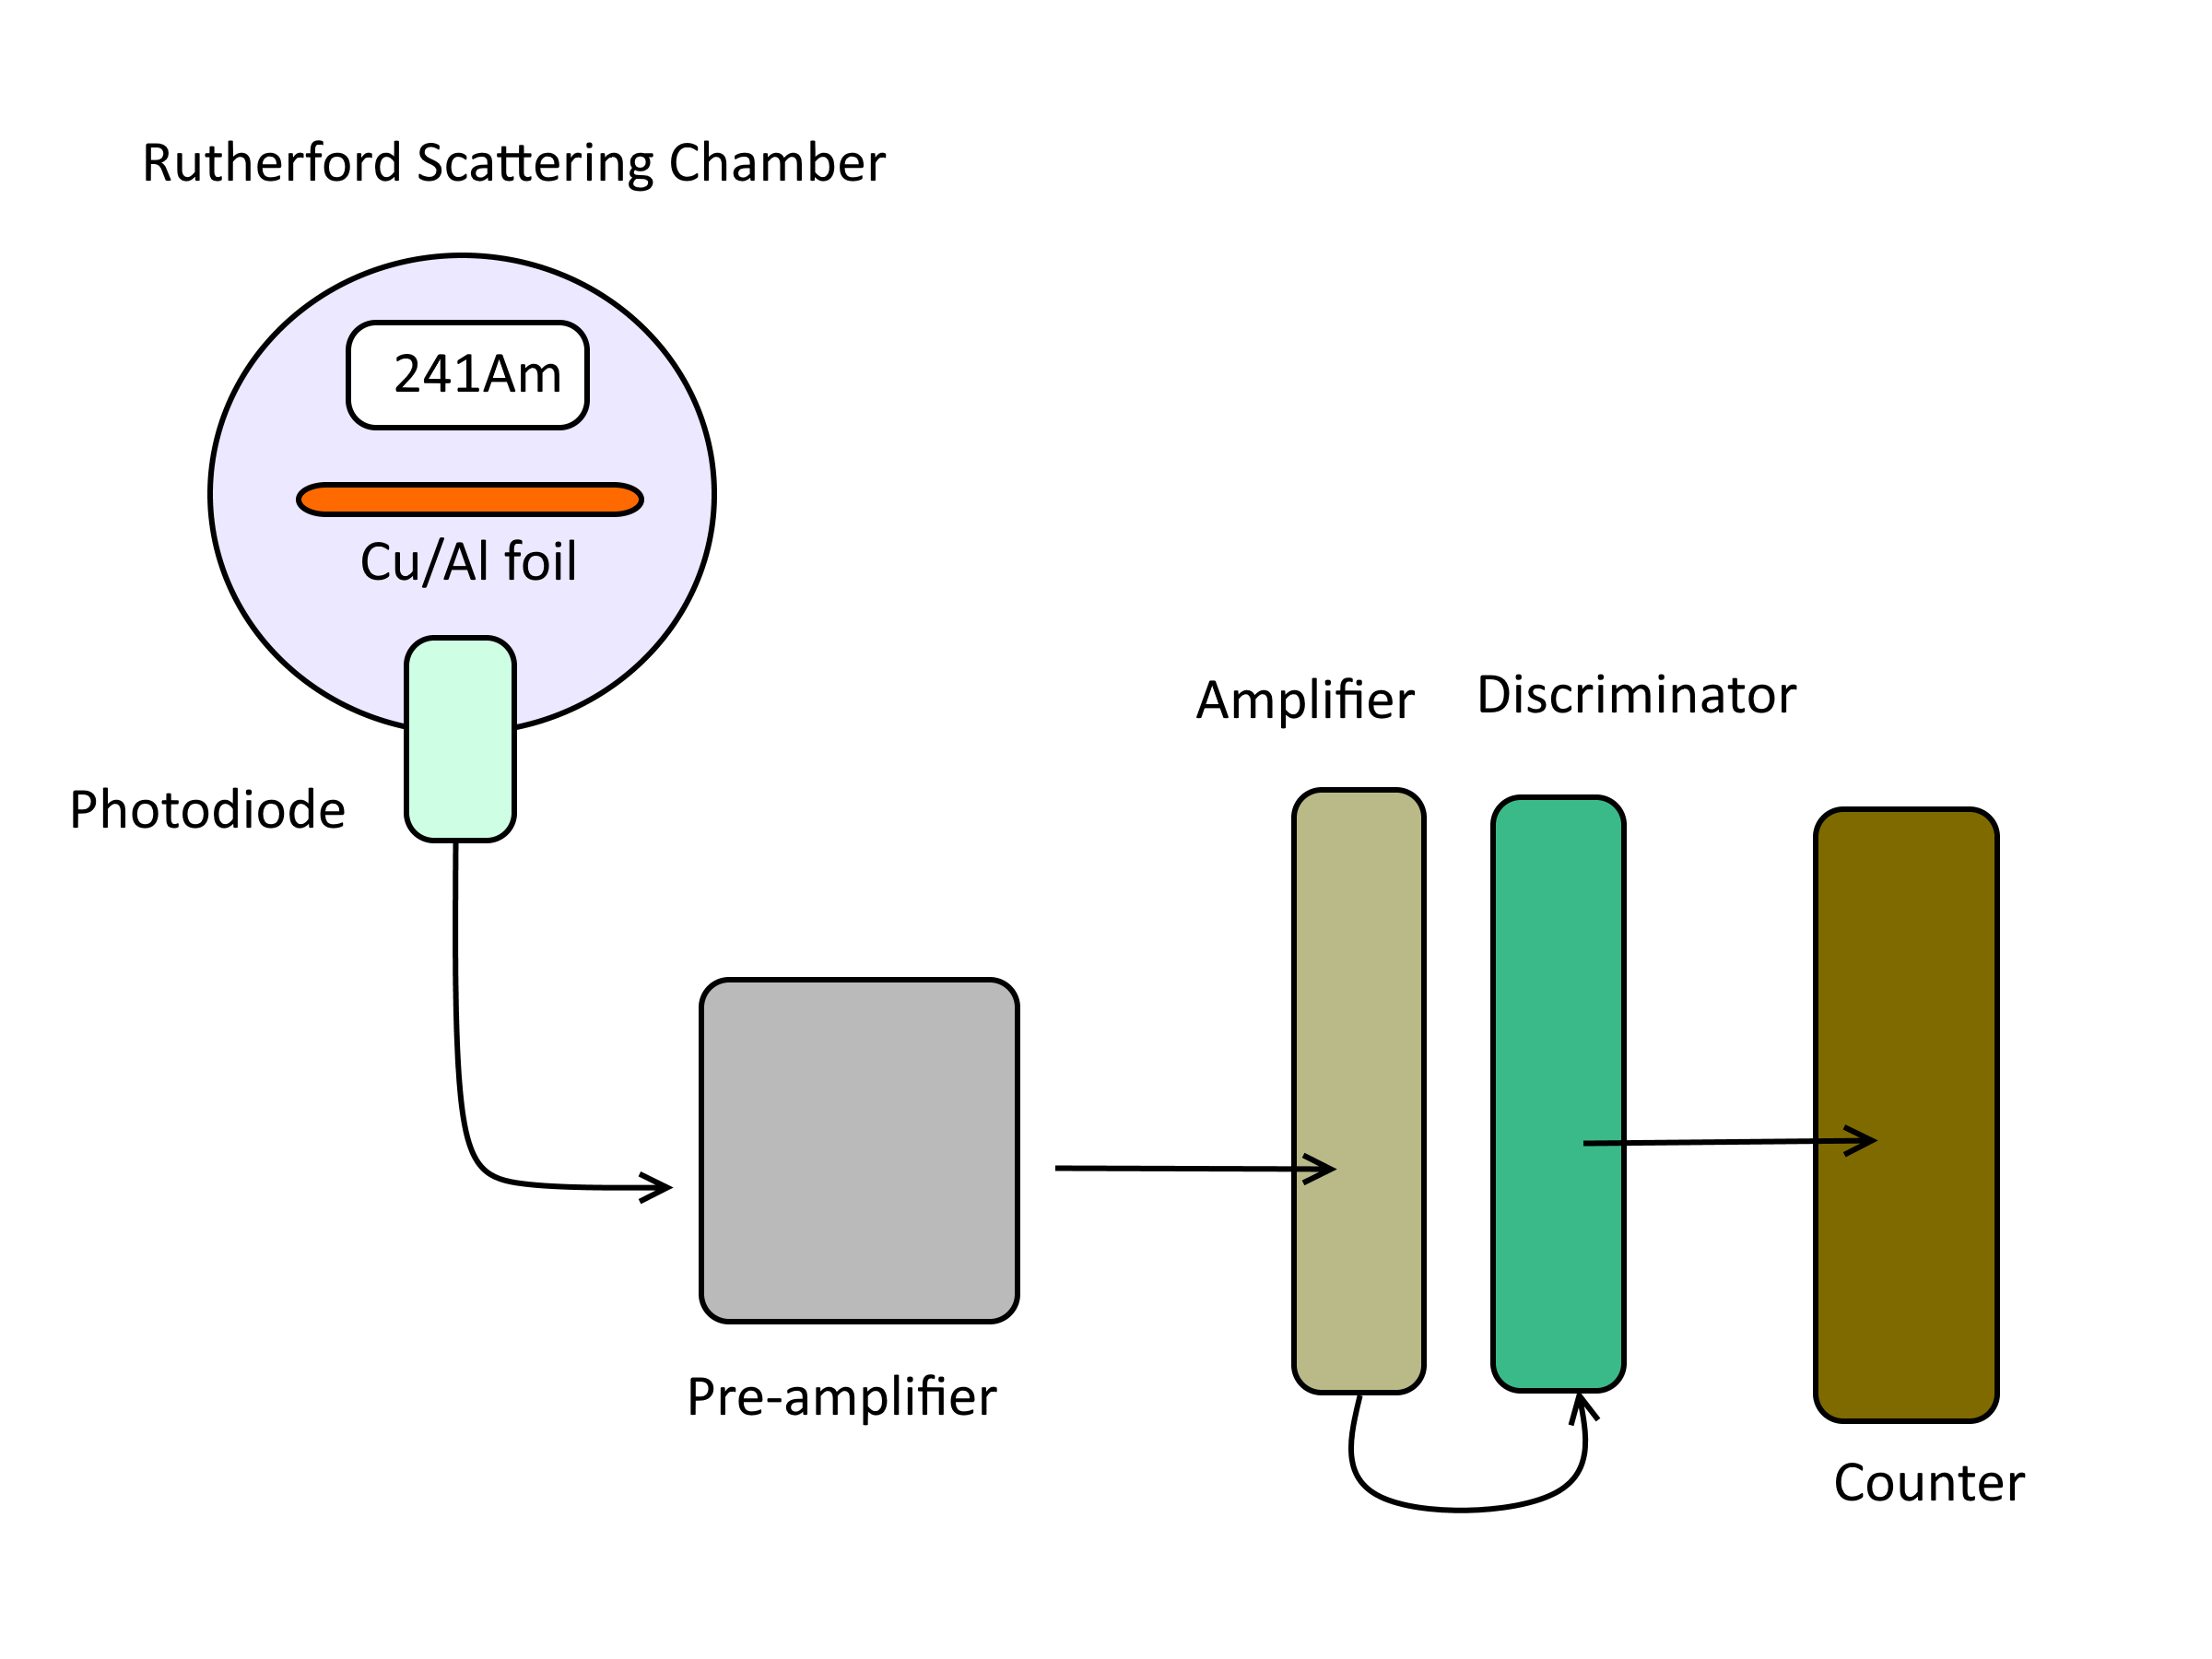
\includegraphics[width=1\textwidth]{diagram.png}
\captionof{figure}{Schematic for circuit diagram }
\label{Diagram}
\end{figure}

\section{Procedure}

% Describe the main steps in the experimental procedures. Be sure to include any
% precautions. Sufficient details should be given such that another student can
% follow and do the experiment.

\subsection{Procedural Modifications}
\qq 

\section{Data Analysis}

%Graphs, figures, and tables with captions
%Results with error analysis
%Calculate discrepancies from theory

\section{Results}

\subsection{Source of Error}

\section{Conclusion}
%Brief summary, discussion of theory

\newpage

P6: Blackbody Radiation

\newpage

\section{Objective of the Experiment}
%A brief statement on the main purpose of the experiment
\qq An incandescent light bulb is used in this experiment as an example of a blackbody radiator. The emission spectrum of the light bulb was measured for various temperatures. The peak wavelength of each emission spectrum was compared to a theoretical peak wavelength, derived using Wien's law and a calculated temperature of the bulb.

\section{Theory of the Experiment}

\qq Any object with nonzero temperature emits electromagnetic radiation. An idealized version of such an object is a "blackbody", which is a perfect absorber and emitter of radiation for all wavelengths. The distribution of emitted thermal energy depends only on the temperature of the blackbody. The temperature of the blackbody can be varied by changing the voltage, and therefore the intensity, of the light bulb. Thus, a series of emission spectra can be produced for a series of temperatures. When relative intensity is plotted against wavelength, a blackbody emission curve is produced that follows Planck's radiation law, given by equation \ref{eq:planck_law}, where $c$ is the speed of light, $k$ is Boltzmann's constant, $T$ is the temperature of the blackbody, and $\lambda$ is the wavelength of the electromagnetic radiation.

\begin{equation}
\label{eq:planck_law}
I \left( \lambda \right) = 
\frac{2 \pi c^2 h}{\lambda^5}
\left( \frac{1}{e^{\frac{hc}{\lambda k T} - 1}} \right)
\end{equation}

\qq The peak of this distribution is given by Wien's law, seen in equation \ref{eq:wien}. Here, the temperature $T$ is the temperature of the bulb filament. This will be calculated from the voltage and current through the bulb in the data analysis section.

\begin{equation}
\label{eq:wien}
\lambda_{max} = \frac{0.002898 \: mK}{T}
\end{equation}

\section{Equipment Utilized}
%List principal pieces of apparatus used by manufacturer, model and
%serial number. When it may be important, list principal
%specifications of certain pieces of equipment (e.g. the focal length
%of an optical system, etc.)

% Description of set-up in prose
\qq The equipment is mounted on the optics bench. The light source is fixed to one end of the bench, and a prism is oriented such that the light source is incident on its apex. The light sensor is attached to a rotating arm, mounted over a labeled disk used to determine the angle of the configuration. In front of the sensor is a collimating lens and collimating slit, separated by a distance equal to the focal length of the lens. \\

Below is a list of some of the key pieces of equipment used in this experiment:

% List of specs
\begin{itemize}
\item Optics bench, used to mount equipment
\item Prism spectrophotometer kit, including collimating slits
\item Broad spectrum light sensor
\item Pasco Capstone software for data acquisition
\item Multimeters, for current and voltage measurements
\end{itemize}

%Labeled sketch of the experimental setup
\begin{figure}[H]
\centering
% uncomment the line below to add image
%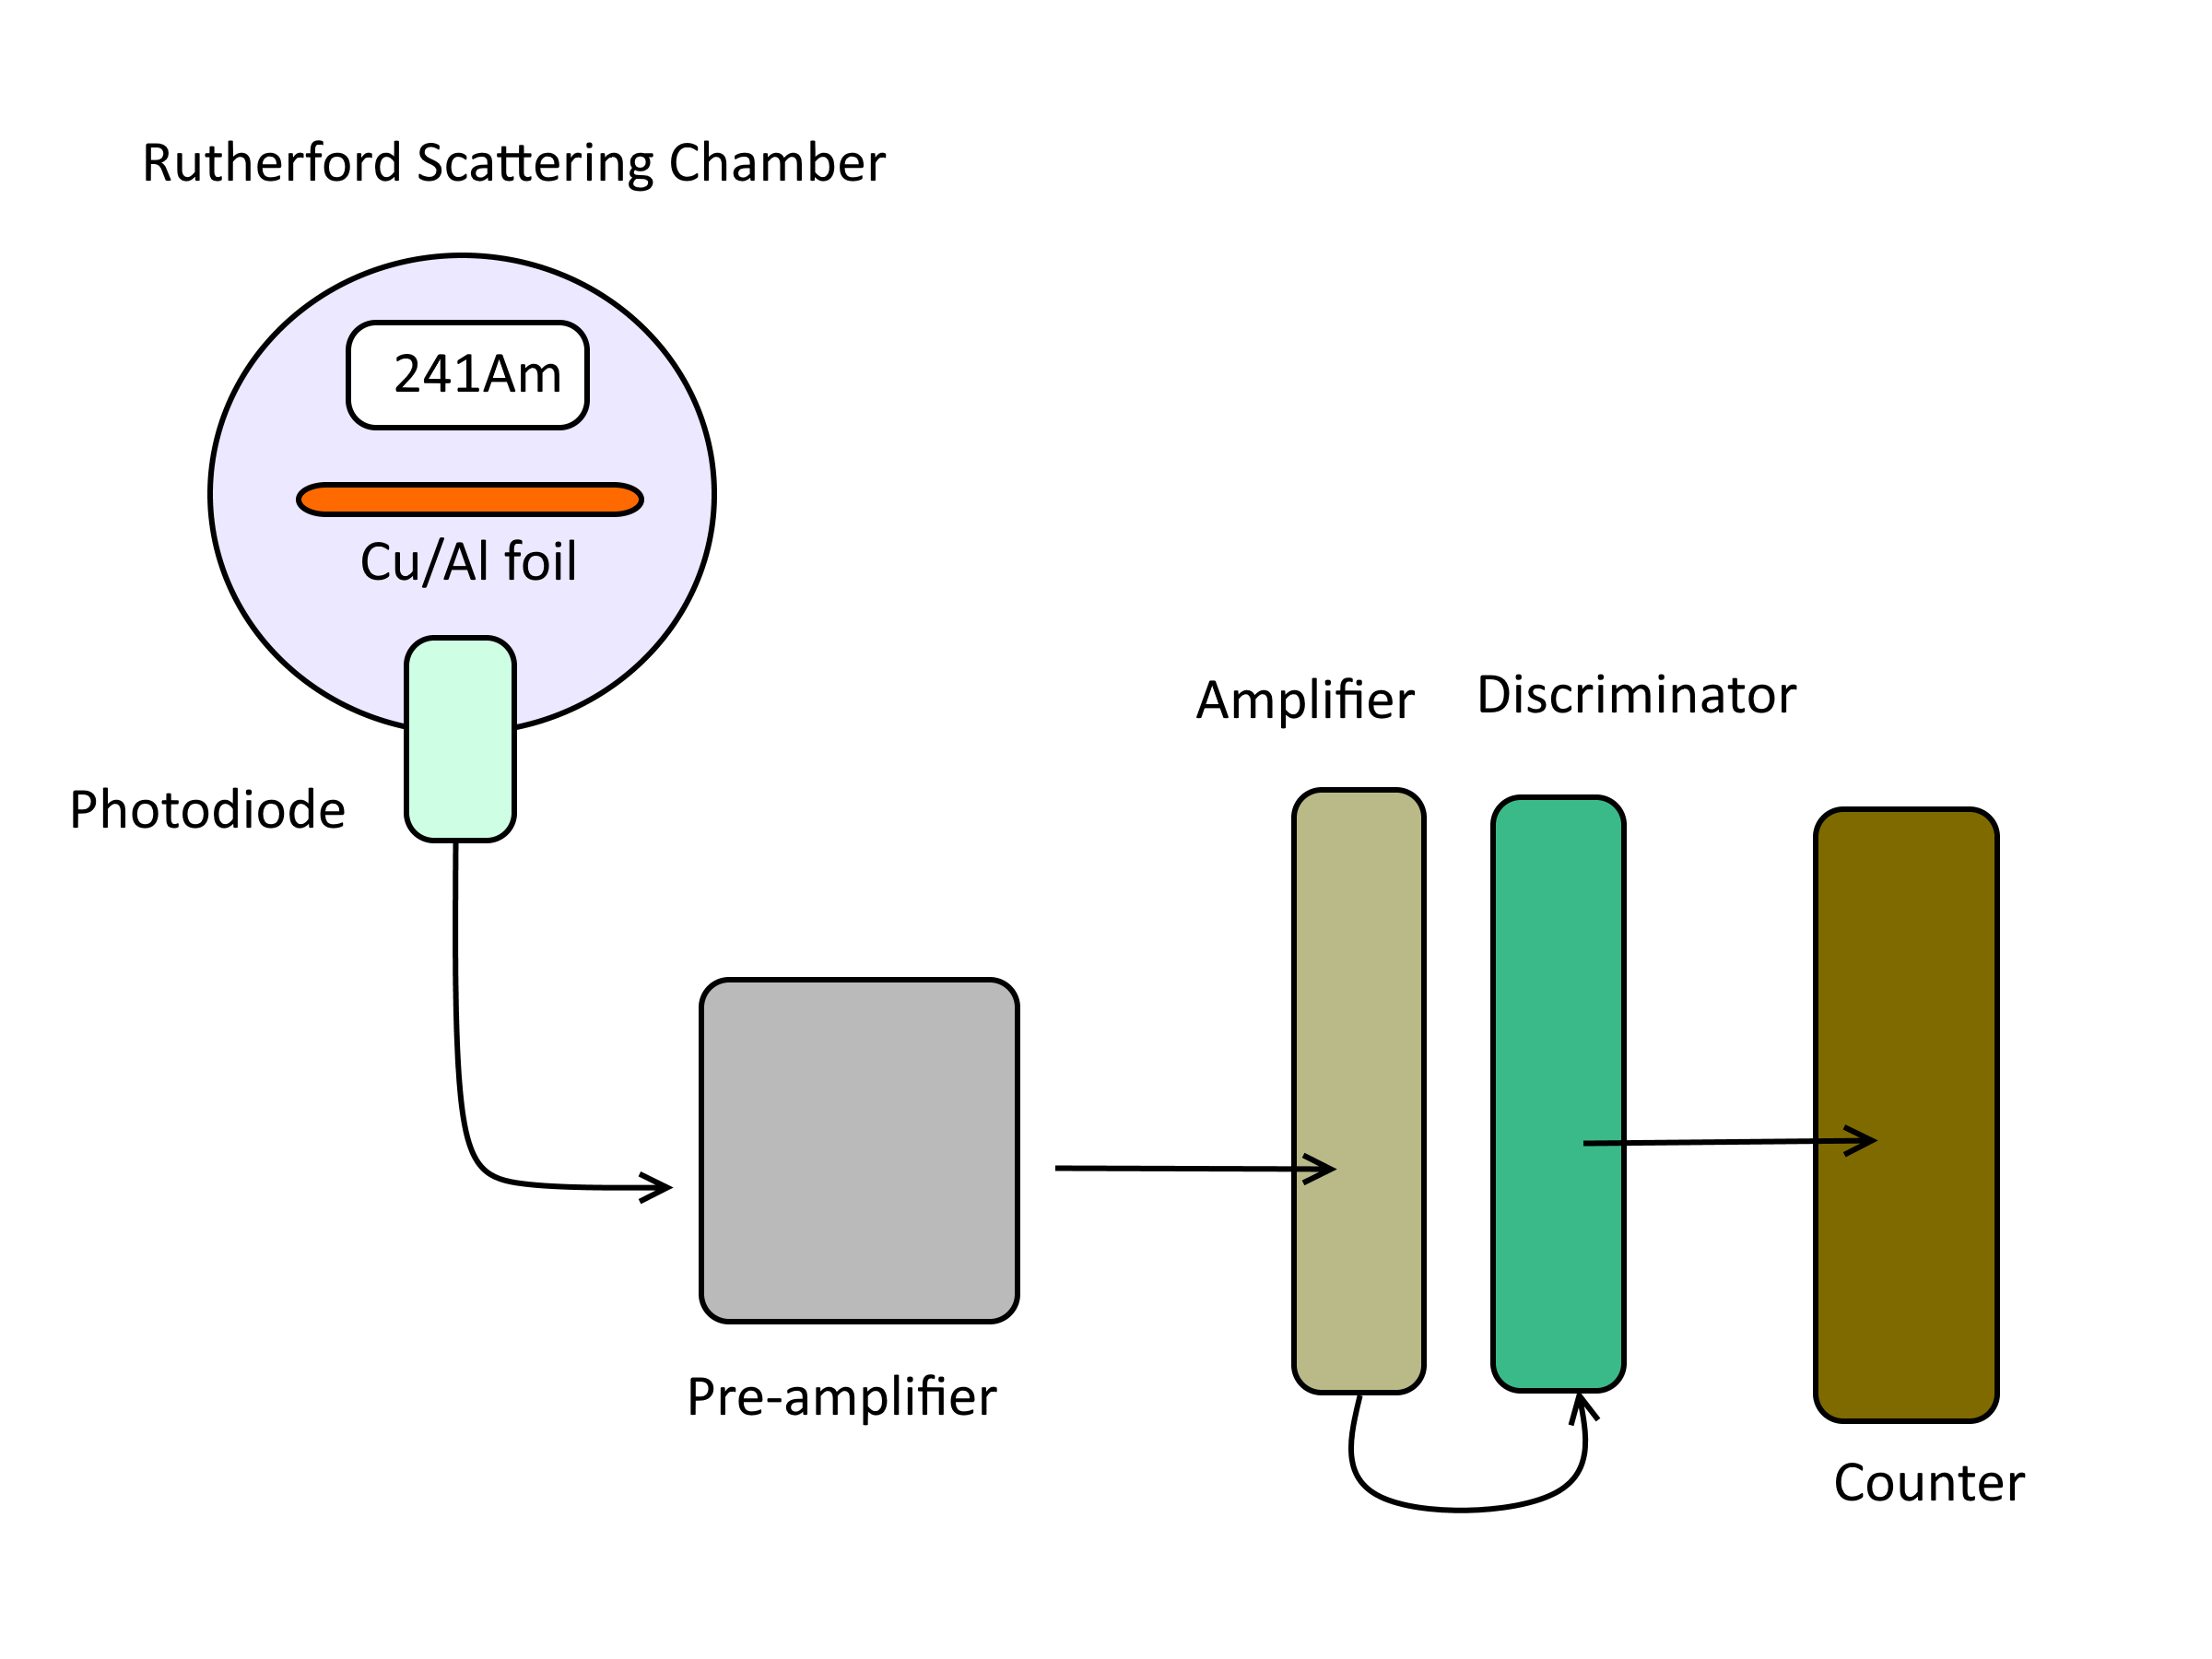
\includegraphics[width=1\textwidth]{diagram.png}
\captionof{figure}{Schematic for circuit diagram }
\label{Diagram}
\end{figure}

\section{Procedure}
% Describe the main steps in the experimental procedures. Be sure to include any
% precautions. Sufficient details should be given such that another student can
% follow and do the experiment.

\qq By having the "blackbody" light source incident on the prism, this set-up allows the entire spectrum to be measured without running into issues caused by diffraction grating. Based on the geometry of the prism, Snell's law will be used to determine the index of refraction, and therefore the wavelength of the incident light (discussed further in the data analysis section). For each incident angle, the corresponding relative intensity is measured with a spectrophotometer, connected to the Pasco Capstone data acquisition software. The spectrophotometer is grounded to the power supply being used to power the light bulb. Two multimeters are used to monitor the current and voltage of the light bulb. The applied voltage was limited to 10 volts to avoid damaging the bulb. The angle was changed in increments of one degree in order to scan through the resultant emission spectrum.

\subsection{Procedural Modifications}
\qq 

\section{Data Analysis}
%Graphs, figures, and tables with captions
%Results with error analysis
%Calculate discrepancies from theory

\qq As the temperature of the light bulb is lowered, the peak of the blackbody curve shifts towards [HIGHER/LOWER] wavelength. Equation \ref{eq:wien} predicts that a lower temperature corresponds to a peak in the longer/greater wavelength spectrum, since the wavelength is inversely proportional to the temperature. Experimental data indicated that as temperature of the light bulb was lowered, the overall intensity of the distribution [INCREASES/DECREASES]. Planck's radiation law also theorizes that decreasing temperature corresponds to decreasing intensity, since the two quantitites are directly proportional.

\qq The temperature of the light bulb filament must be calculated from the measured voltage and current for each trial. The resistance of the filament is first determined using a modified form of Ohm's law, $R=V/I$. Resistivity, $r$, can be calculated from this resistance using equation \ref{eq:resistivity}, where $r_0 = 5.65 \mu \Omega cm$ is the resistivity of Tungsten at room temperature, $R_{bulb}=0.93 \Omega$ is the resistance of the bulb, and $V/I$ is the calculated resistance of the filament. 

\begin{equation}
\label{eq:resistivity}
r =
\left(
\frac{\frac{V}{I}-0.2}{R_{bulb}}
\right)
\end{equation}

A sample calculation is shown below for the case of an applied voltage of $3V$:
\begin{align*}
r &=
\left(
\frac{\frac{3}{0.388}-0.2}{0.93}
\right) \\
&= 45.8 \; \mu \Omega cm
\end{align*}

Temperature was calculated from resistivity using the following fit equation:
$$T[K] = 103 + 38.1r - 0.095r^2 = (2.48\times 10^{-4}) r^3$$
For the $3V$ case discusses above, for example, the temperature was determined to be $1671K$. From the temperature of the filament, Wien's law is used to determine a theoretical value of $\lambda_{peak}$.

\begin{center}
\begin{tabular}{|c|c|c|}
\hline 
Voltage & Temperature & Theoretical $\lambda_{peak}$ \topVspace \bottomVspace \\
\hline
3V & 1671 K & $1.73 \times 10^{-6}$ m \\
5V & TEMP K & WAV m\\
7V & TEMP K & WAV m\\
9V & TEMP K & WAV m\\
\hline
\end{tabular}
\label{table:temps}
\captionof{table}{Calculated temperature of light bulb filament for each applied voltage; this is used to determine theoretical peak wavelength}
\end{center}

\section{Results}

\subsection{Source of Error}

\section{Conclusion}
%Brief summary, discussion of theory

\section{Appendices}

\end{document}
